\section{Hardware Enhancements}\label{ch:hardware}
The main focus of the enhancements is on the axes and bearings, which were previously 3D-printed and are now replaced with more robust components.
The Yaw joint was also significantly modified, now featuring a planetary gearbox to increase the torque available at the joint.

\subsection{Shoulder Joint}
The shoulder joint is the most complex part of the robotic arm, featuring two degrees of freedom, tilting the arm in two axes.
Most of the parts of this Joint are stationary, meaning they are not moving with the arm.
As a first enhancement, all stationary parts (the side braces and the base plate) were replaced with aluminum components, which are more robust and durable than the previous 
3D-printed parts. The two joint axes of the shoulder joint are driven by servo motors, which drive several gears to achieve the desired range of motion.
There are six gear axes used to fix the gears to the side braces. all of these axes were previously 3D-printed and are now replaced with aluminum components.
Furthermore, all axes of the shoulder joint are now supported by ball bearings, as seen in \autoref{fig:shoulderjoint_improvements}.

\begin{figure}[htbp]
    \centering
    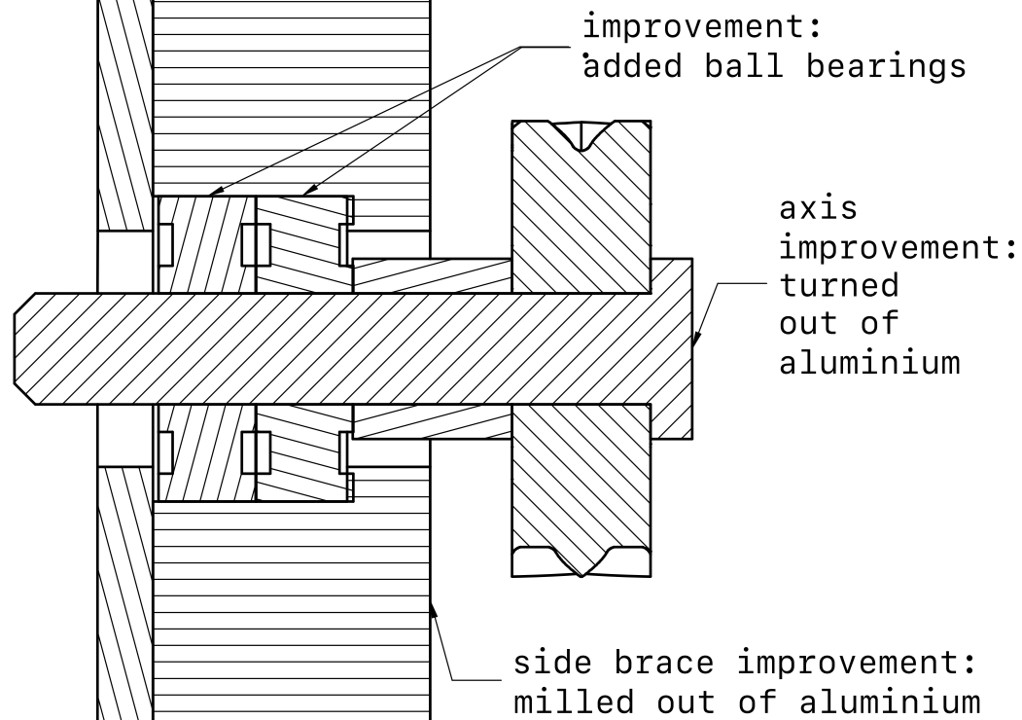
\includegraphics[width=0.8\linewidth]{images/shoulderjoint_improvements.jpg}
    \caption{Examplary view of the improvements made to the shoulder joint, showing the section view of one gear axis.}
    \label{fig:shoulderjoint_improvements}
\end{figure}

The centerpiece of the joint are the four bevel gears, which are the key to allowing the two degrees of freedom. The two fixed gears are mounted to the side braces as mentioned above,
while the two moving gears mount the arm itself. Previously, these gears both had their own axis, fixed to the two sides of the arm respectively. Now, they share a common axis,
where one of them is fixed and the other is free to rotate using ball bearings, as seen in \autoref{fig:bevelaxis_improvements}. This change improves the alignment,
fixing the gears in place in axial direction, negating the need
for tensioning tape as used in the previous assembly\parencite{zeitlerDualArmAerialManipulation}.

\begin{figure}[htbp]
    \centering
    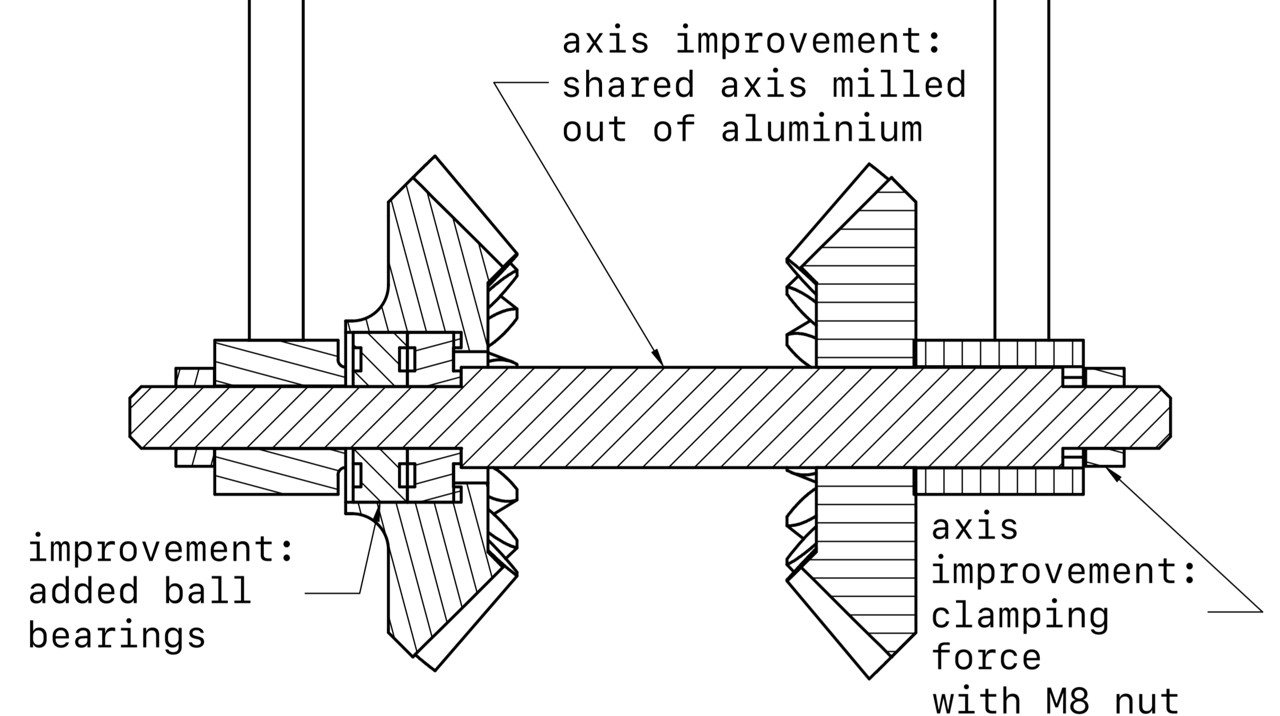
\includegraphics[width=0.8\linewidth]{images/bevelaxis_improvements.jpg}
    \caption{Section view of the improvements made to the bevel axis.}
    \label{fig:bevelaxis_improvements}
\end{figure}

\subsection{Yaw Joint}
The yaw joint is the second joint of the robotic arm, featuring one degree of freedom allowing the arm to rotate around its vertical axis.
Previously, the yaw joint had a 1:1 gear ratio, which was changed to a 8:1 gear ratio to increase the torque available at the joint using a planetary gearbox shown 
in \autoref{fig:planetary_gearbox_section}. This gearbox is made up of a sun gear driven by the motor, three planet gears which drive the rest of the arm, 
and a ring gear fixed to the lower part of the arm. These gears were designed using a gearbox template for OpenSCAD\parencite{thingiverse.comCustomizablePlanetaryGearbox} And 3D-printed at the
workshop of the institute.
The planetary gears themselves are mounted on the carrier using ball bearings marked in blue in the figure, 
the motor axis used to drive the sun gear is marked in black. This axis is also turned out of aluminum to increase durability. The carrier and the gears are 3D-printed.
The axes of the planet gears are made up of screws, which directly connect the carrier to the top part of the arm.

\begin{figure}[htbp]
    \centering
    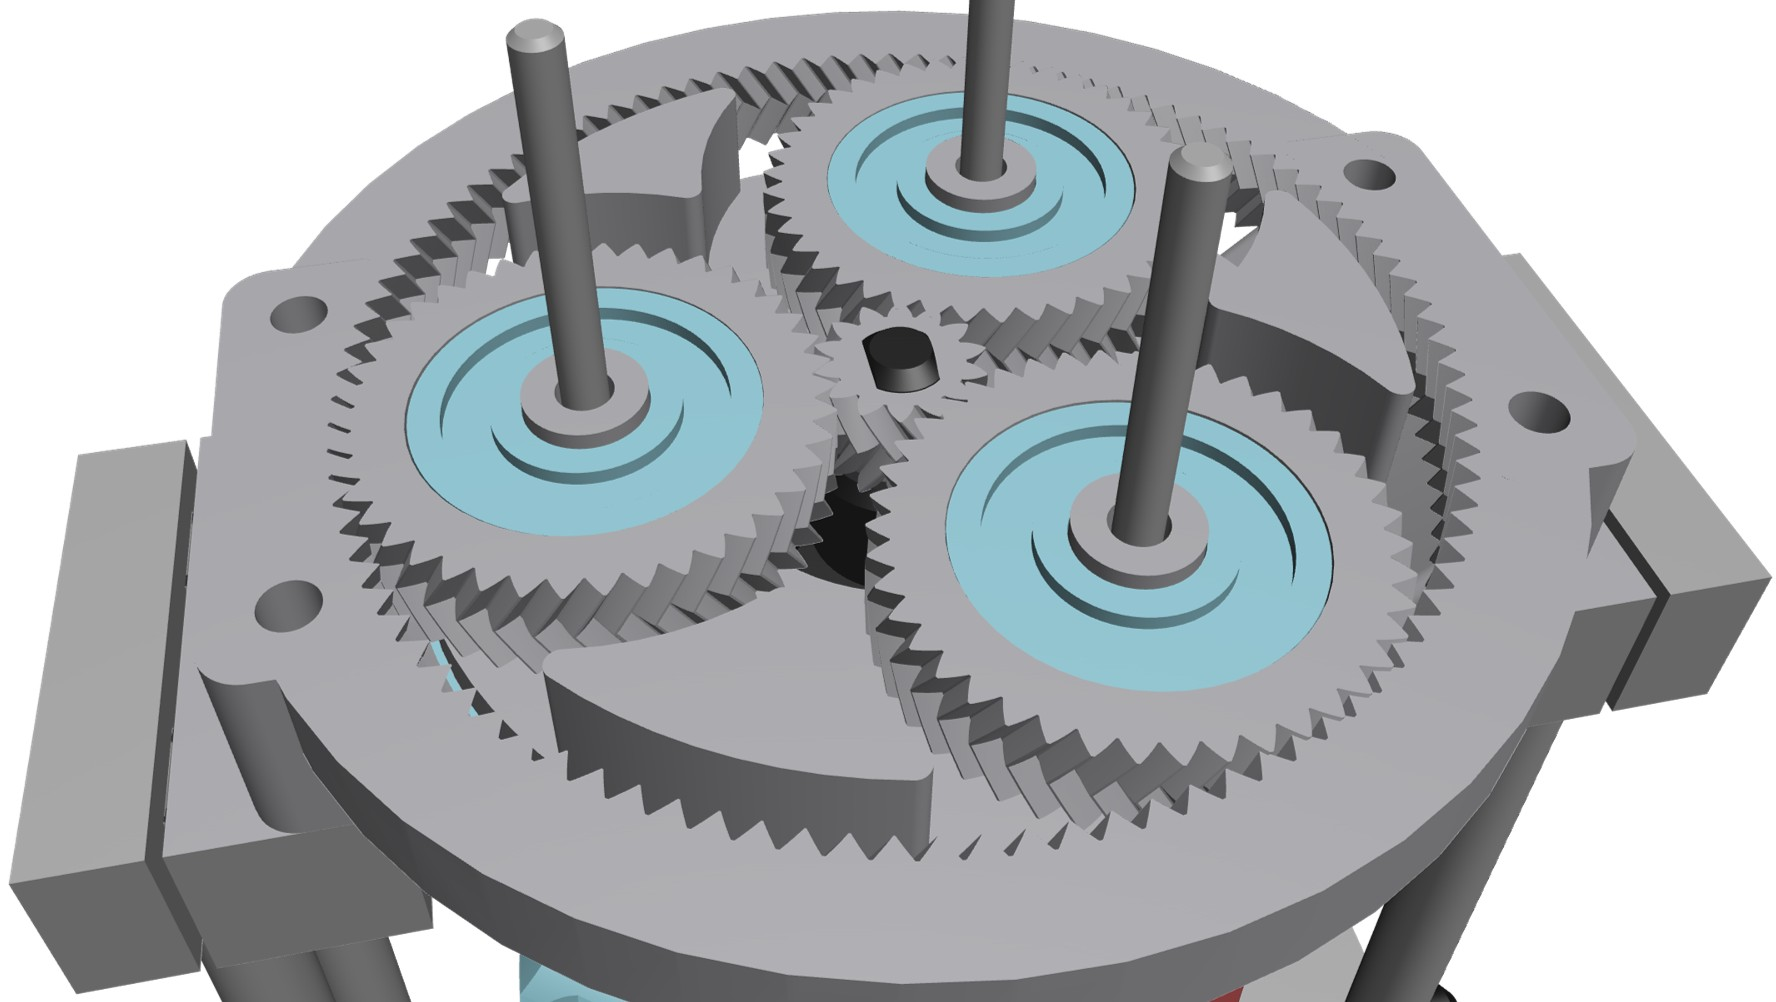
\includegraphics[width=0.8\linewidth]{images/planetary_gearbox_section.jpg}
    \caption{View of the gears in the planetary gearbox.}
    \label{fig:planetary_gearbox_section}
\end{figure}

Furthermore, the axis of the yaw joint is now supported by axial bearings, which improves the precision of the robot. Two axial bearings are used, one above and one below the 
planetary gear carrier. The bearings are marked in blue in \autoref{fig:planetary_gearbox_explosion}.

The four axes marked in \autoref{fig:planetary_gearbox_explosion} show screws, two of which connect the outer gear ring to the base plate of the arm, while the other two
connect the lid of the planetary gearbox to the base plate. For future development, the lid of the planetary gearbox could be fixed using four screws instead of two,
to improve the stability of the construction.

\begin{figure}[htbp]
    \centering
    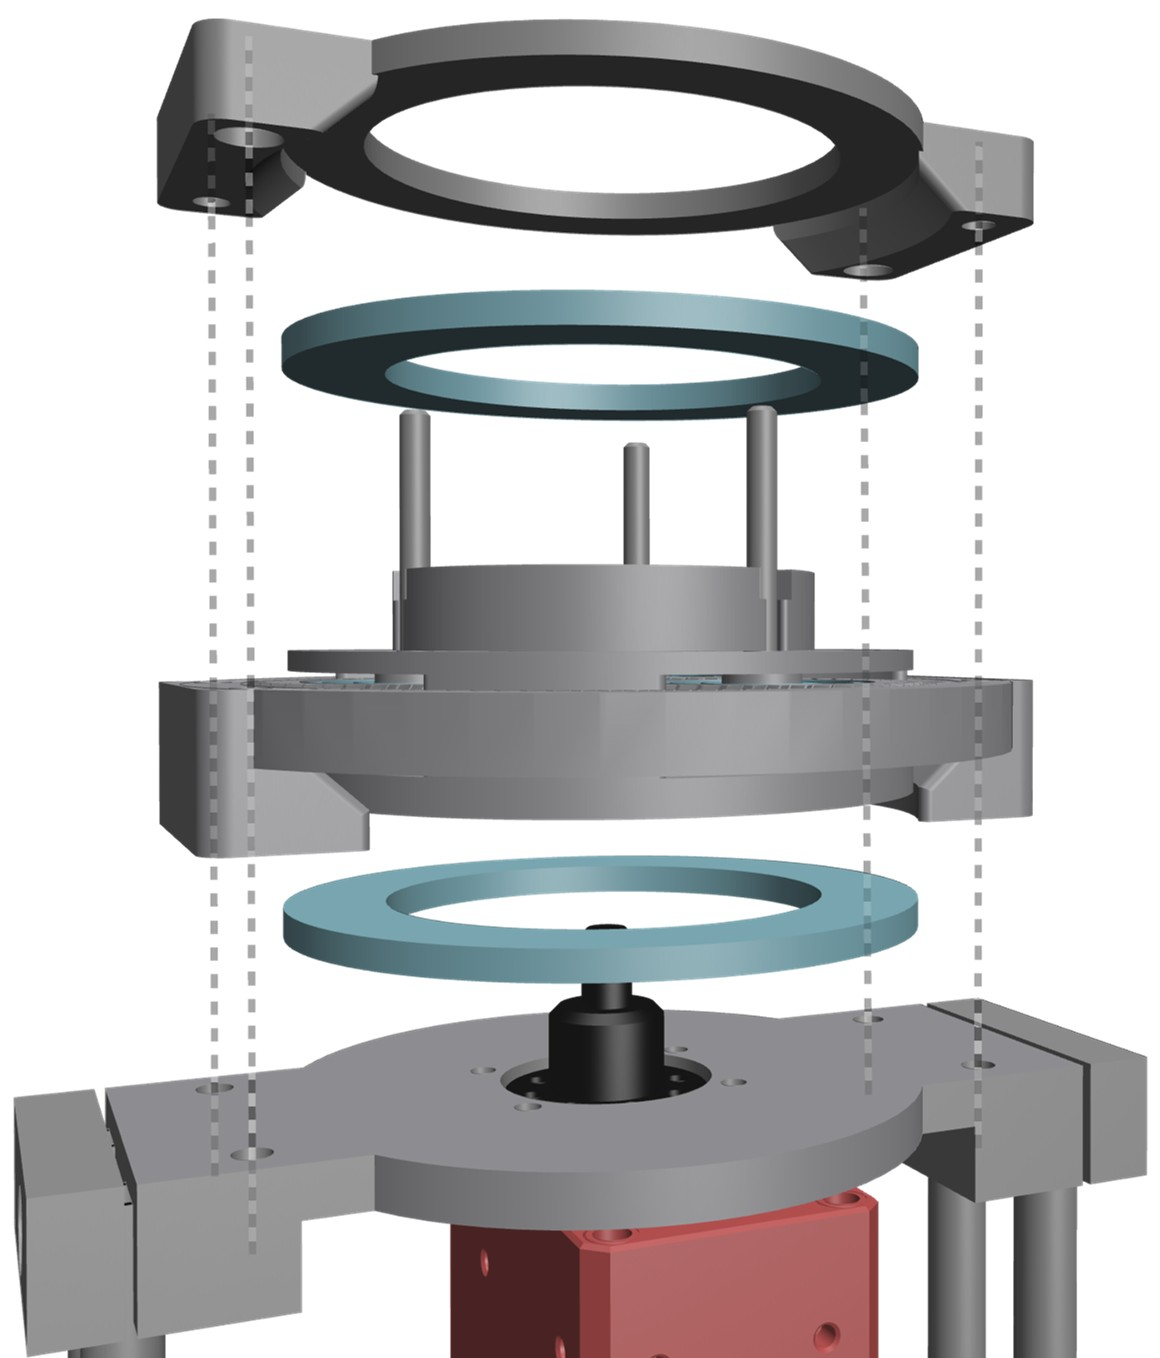
\includegraphics[width=0.8\linewidth]{images/planetary_gearbox_explosion.jpg}
    \caption{Exploded view of the planetary gearbox.}
    \label{fig:planetary_gearbox_explosion}
\end{figure}

To further improve the 3D-printed planetary gearbox, silicone spray was applied to the gears to reduce friction and wear. The impact on the friction was measured using the current
sensor of the servo motor, as the internal friction of the gearbox is directly proportional to the current needed to drive the gearbox. As seen in 
\autoref{fig:planetary_gearbox_assessment}, the application of silicone spray resulted in a slight reduction of measured current, derefore proving a reduction of friction.

\begin{figure}[htbp]
    \centering
    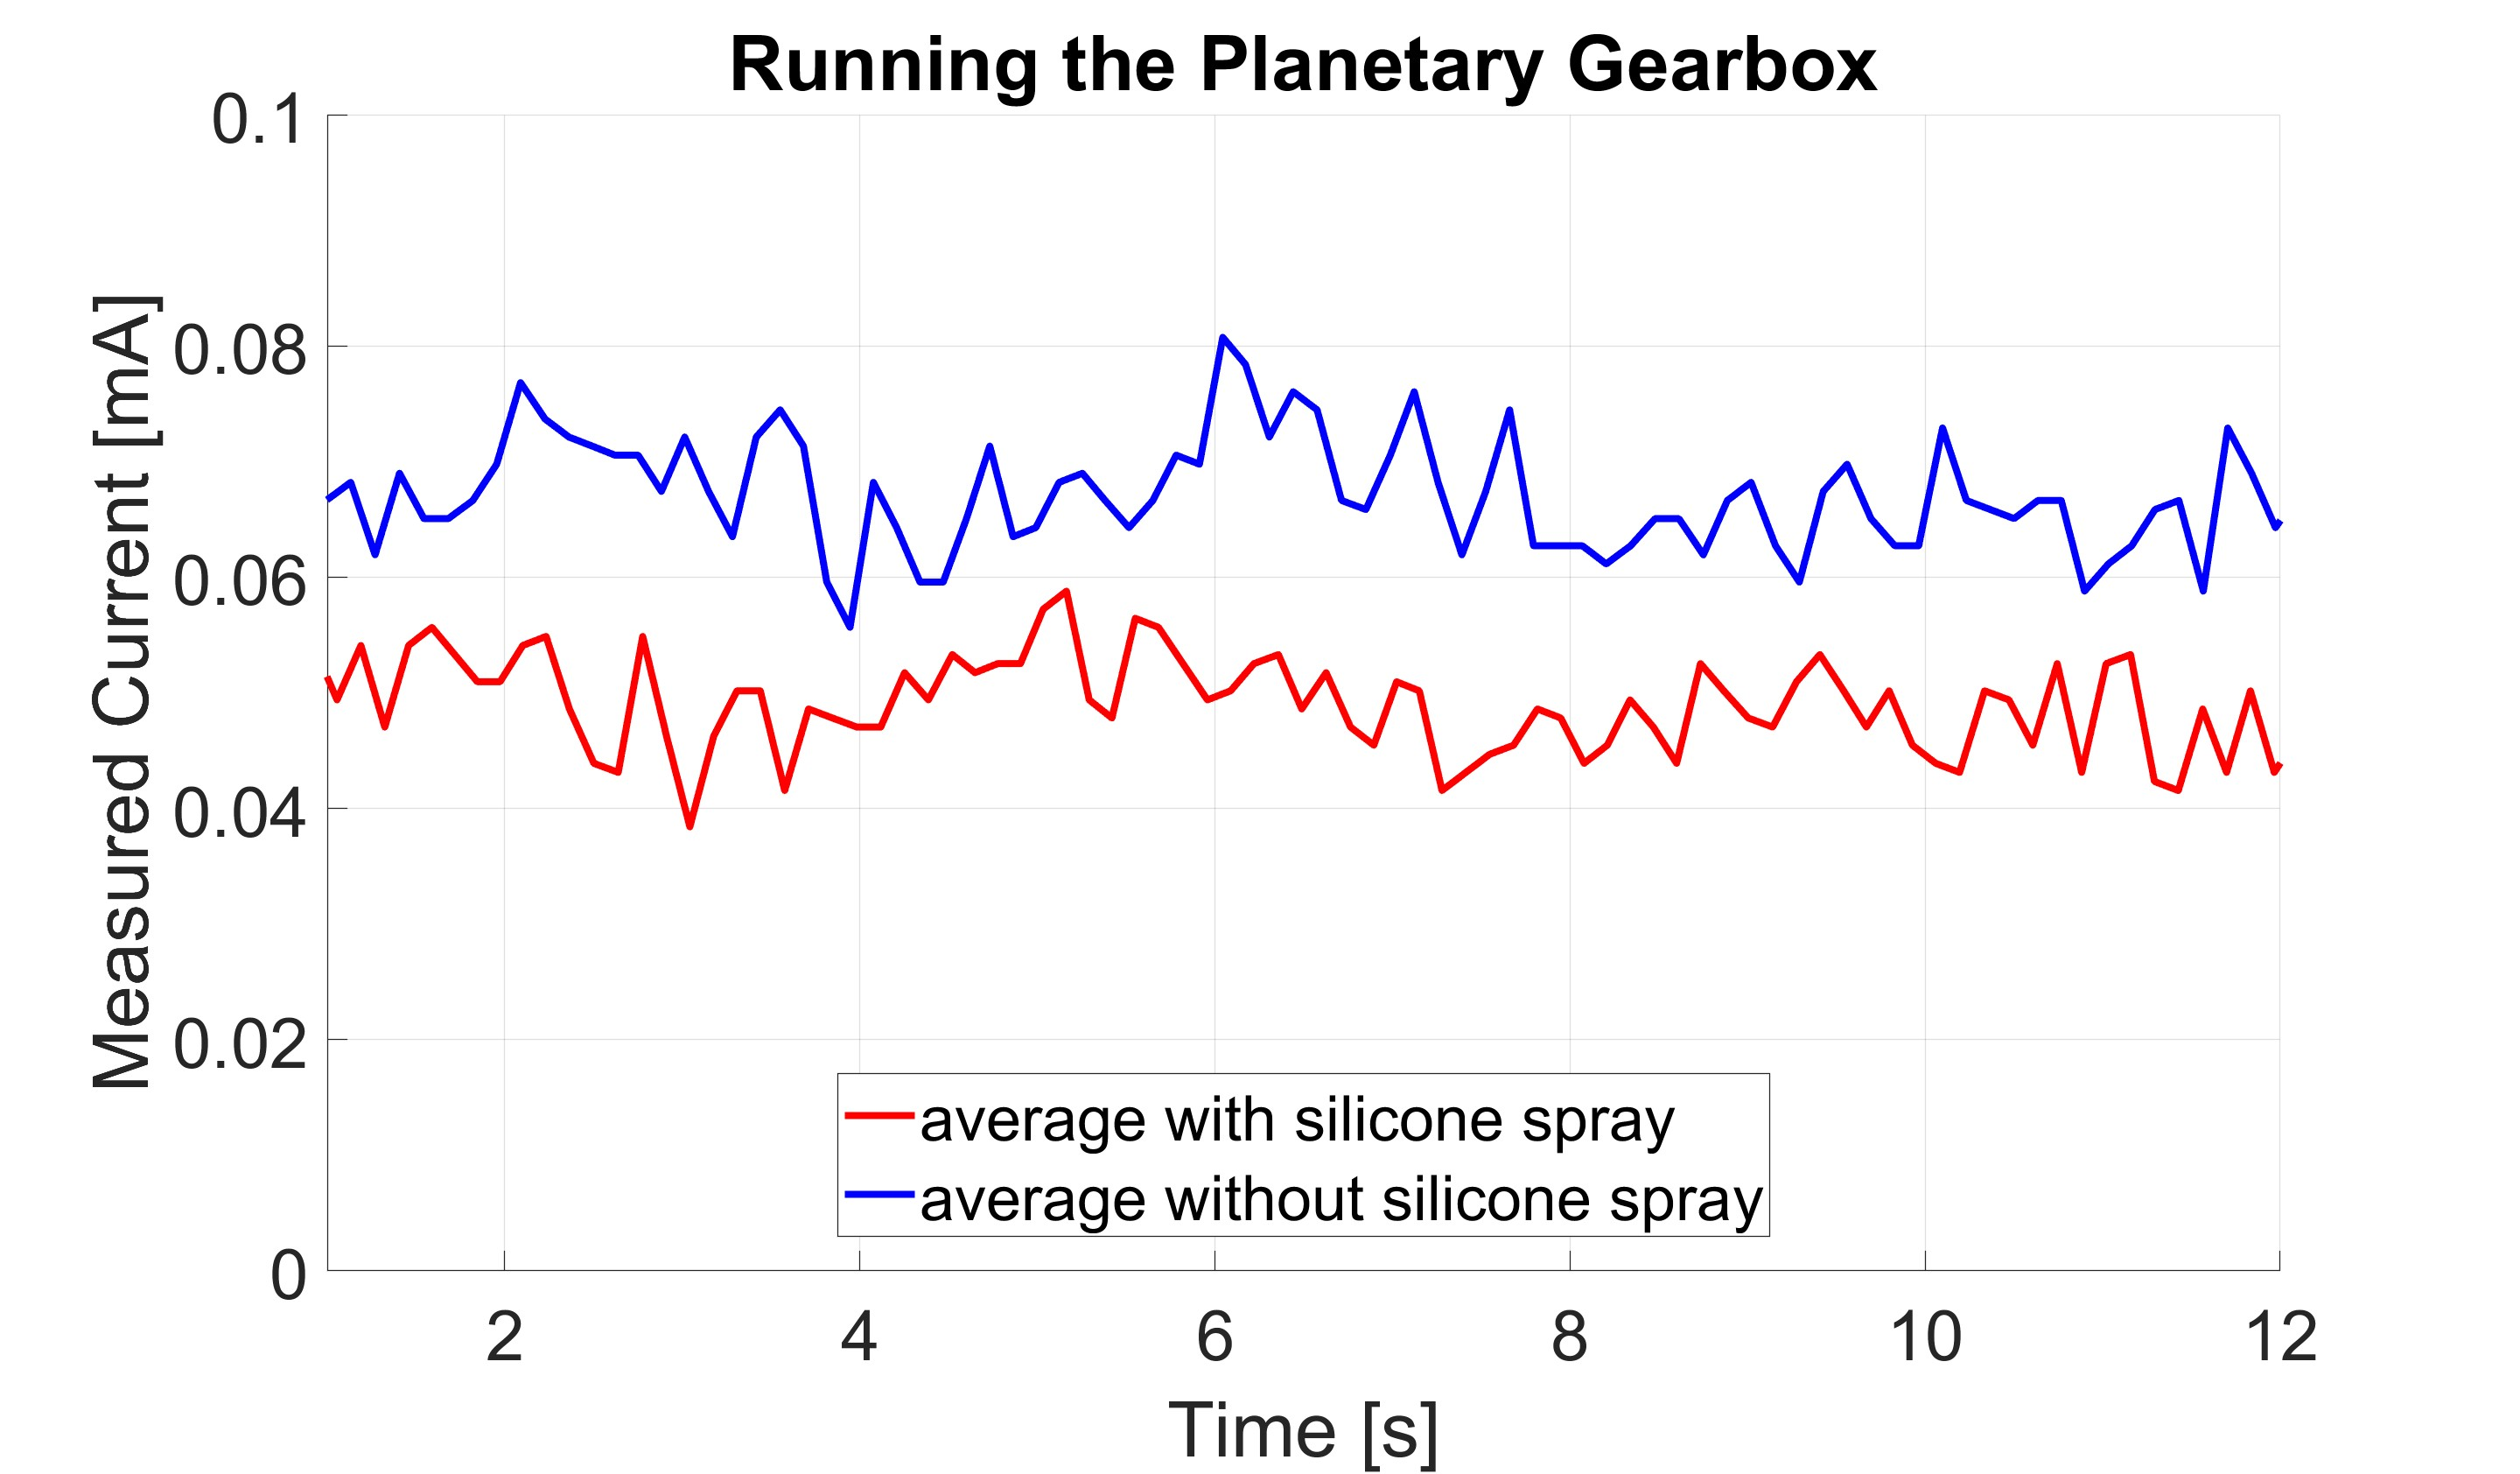
\includegraphics[width=\linewidth]{images/matlab/planetary_gearbox_assessment.jpg}
    \caption{Assessment of the planetary gearbox internal resistance before and after applying silicone spray.}
    \label{fig:planetary_gearbox_assessment}
\end{figure}

For future developments, one possible improvement in terms of assembly could be to substitute the three screws used as planet gear axes with screws featuring a hexagon head,
and adapt the bottom plate of the planetary gear carrier in such a way that the screwheads are locked in position and the screws cannot turn. This would ease the assembly process,
as the screws would not need to be held in place while tightening the nuts on the other side.

\subsection{Elbow Joint}
The elbow joint is the third joint of the robotic arm, featuring one degree of freedom allowing the arm to bend.
This joint is driven by a belt drive, for which the gears where previously 3D-printed and are now replaced with commercially available aluminum gears.
Two axes are part of this joint, one motor axis which drives the belt and one output axis to drive the arm. Both of these are replaced with aluminum axes.

The motor axis is now supported by two ball bearings as seen in \autoref{fig:motoraxis_improvements}. The connecting piece which holds the motor axis
connects to carbon fiber rods which continue upwards. This connection now introduces a clamping mechanism instead of the previous glue connection for better modularity.

\begin{figure}[htbp]
    \centering
    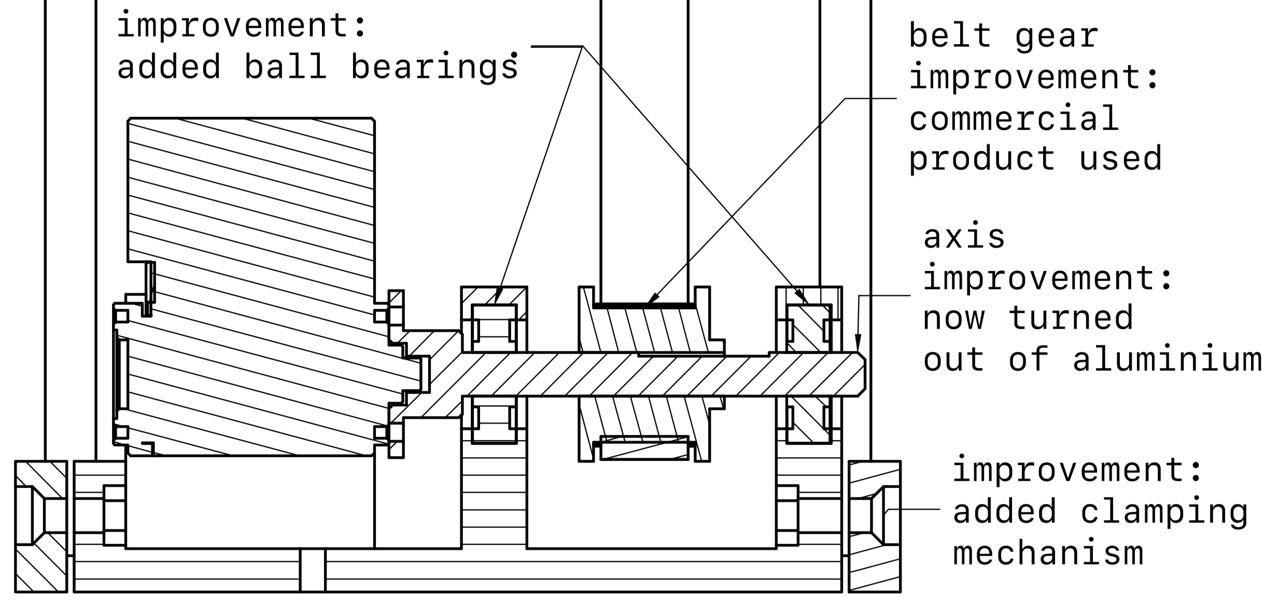
\includegraphics[width=0.8\linewidth]{images/motoraxis_improvements.jpg}
    \caption{Section view of the construction surrounding the motor axis.}
    \label{fig:motoraxis_improvements}
\end{figure}

The elbow axis sits at the other end of the belt drive, and is therefore responsible for tensioning the belt. This tensioning mechanism consists of screws and self-securing nuts,
supporting the ball bearings and applying the necessary force to keep the belt tentioned, see \autoref{fig:elbowaxis_improvements}

\begin{figure}[htbp]
    \centering
    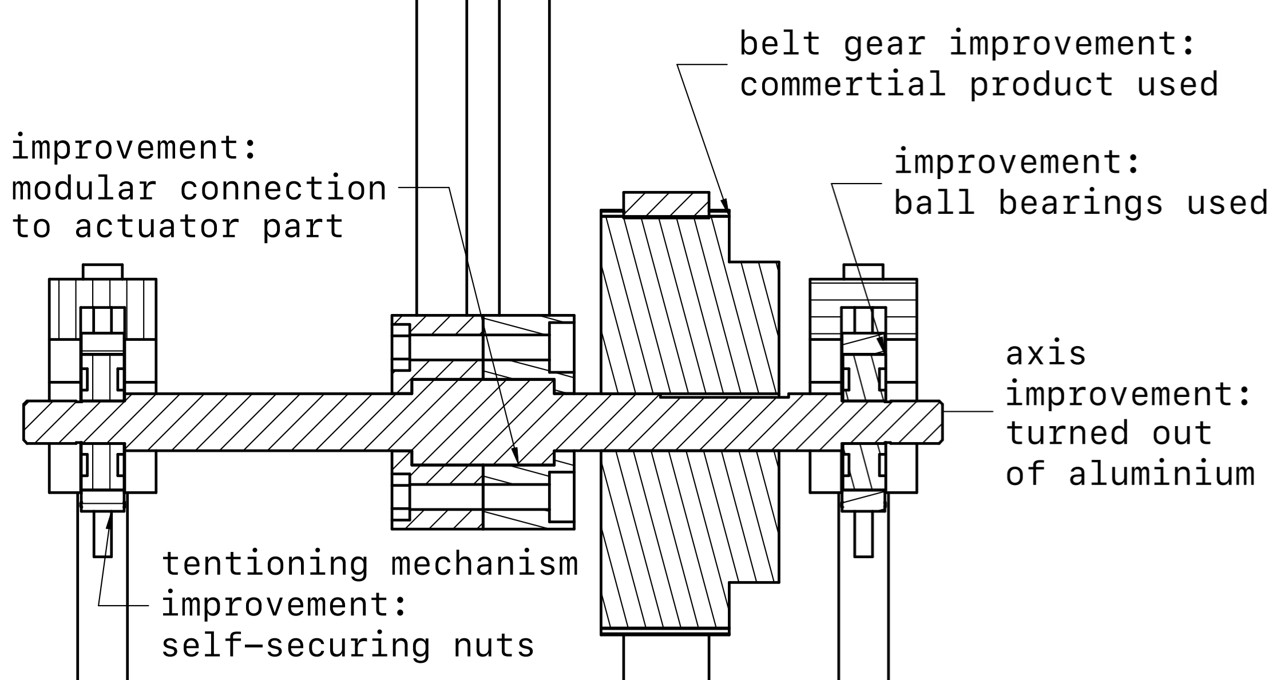
\includegraphics[width=0.8\linewidth]{images/elbowaxis_improvements.jpg}
    \caption{Section view of the construction surrounding the elbow axis.}
    \label{fig:elbowaxis_improvements}
\end{figure}

For future development, the connection to the actuator part (see \autoref{fig:elbowaxis_improvements}) could be constructed to have a larger overlap between
the aluminum axis and the 3D-printed carbon fiber rod holder. This would reduce the endpoint force of the aluminum pressing against the 3D-printed part.
Reducing this force will reduce the wear in the 3D-printed part, which is responsible for end-effector inaccuracies. The current solution to this inaccuracy problem is epoxy glue,
however this reduces the modularity.
Another improvement could be to increase the length of the housing around the tensioning mechanism. Currently, the self-securing nuts do not overlap with the housing.
This leads to the possibility of these nuts to turn in place, as the current fastening method is not secure enough, glue is needed in the current design to hold these nuts in place.
If the housing were to overlap with the screws, it would prevent them from turning freely, fixing this problem
without the need for glue. 

\subsection{End-Effector}
The end-effector (TCP) is the last part of the robotic arm, which is used to interact with the environment.
To easily exchange the end-effector, the clamping mechanism introduced in \autoref{fig:motoraxis_improvements} is used here as well to connect the end-effector to the carbon fiber rods.
The current design features a the two-fingered gripper manufactured by makeblock\parencite{makeblockDatenblattMakeblockRobotergreifer} as seen in \autoref{fig:gripper}. 

\begin{figure}[htbp]
    \centering
    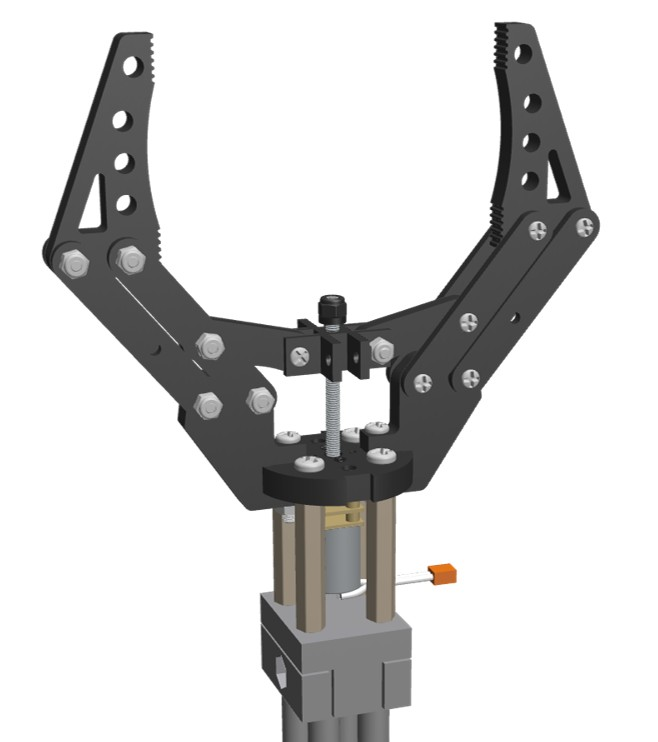
\includegraphics[width=0.8\linewidth]{images/gripper.jpg}
    \caption{Robot end-effector featuring a simple gripper.}
    \label{fig:gripper}
\end{figure}

Since the PCB board used in this project only supports dynamixel servos and no external motors, the gripper is controlled manually using a switch at the base of the robot arm.
%For this, the dynamixel power supply board's 5V output is used in combination with a double-pole double-throw (DPDT) switch to reverse the polarity of the voltage applied to the
%gripper motor as seen in \autoref{fig:gripper_circuit}.

%\begin{figure}[htbp]
%    \centering
%    \begin{circuitikz}
%        \draw
%        (0,2) node[left]{5V} to [short, o-] (0.5,2)
%        (0,0.5) node[left]{GND} to [short, o-] (0.5,0.5)
%        (1,2) node[spdt] {}
%        (1,0.5) node[spdt] {}
%        (1.5,1.685) to [short, -] (3,1.685) to[short, -o] (3,0.815)
%        (1.5,0.815) to [short, -] (5,0.815)
%        (5,0.815) to[Telmech=M] (5,2.315)
%        (1.5,2.315) to [short, -] (5,2.315)
%        (1.5,0.185) to [short, -] (3.5,0.185) to[short, -o] (3.5,2.315)
%        ;
%        \draw [dashed] (1,2.1) to [short] (1,0.6);
%    \end{circuitikz}
%    \caption{Circuit diagram of the manual gripper control.}
%    \label{fig:gripper_circuit}
%\end{figure}

For future development, a different microcontroller could be used to incorporate gripper control into the software.

\subsection{Construction}
With all hardware enchancements made, the improved version of the robotic arm can be seen in \autoref{fig:robot_arm_final}.
\begin{figure}[htbp]
    \centering
    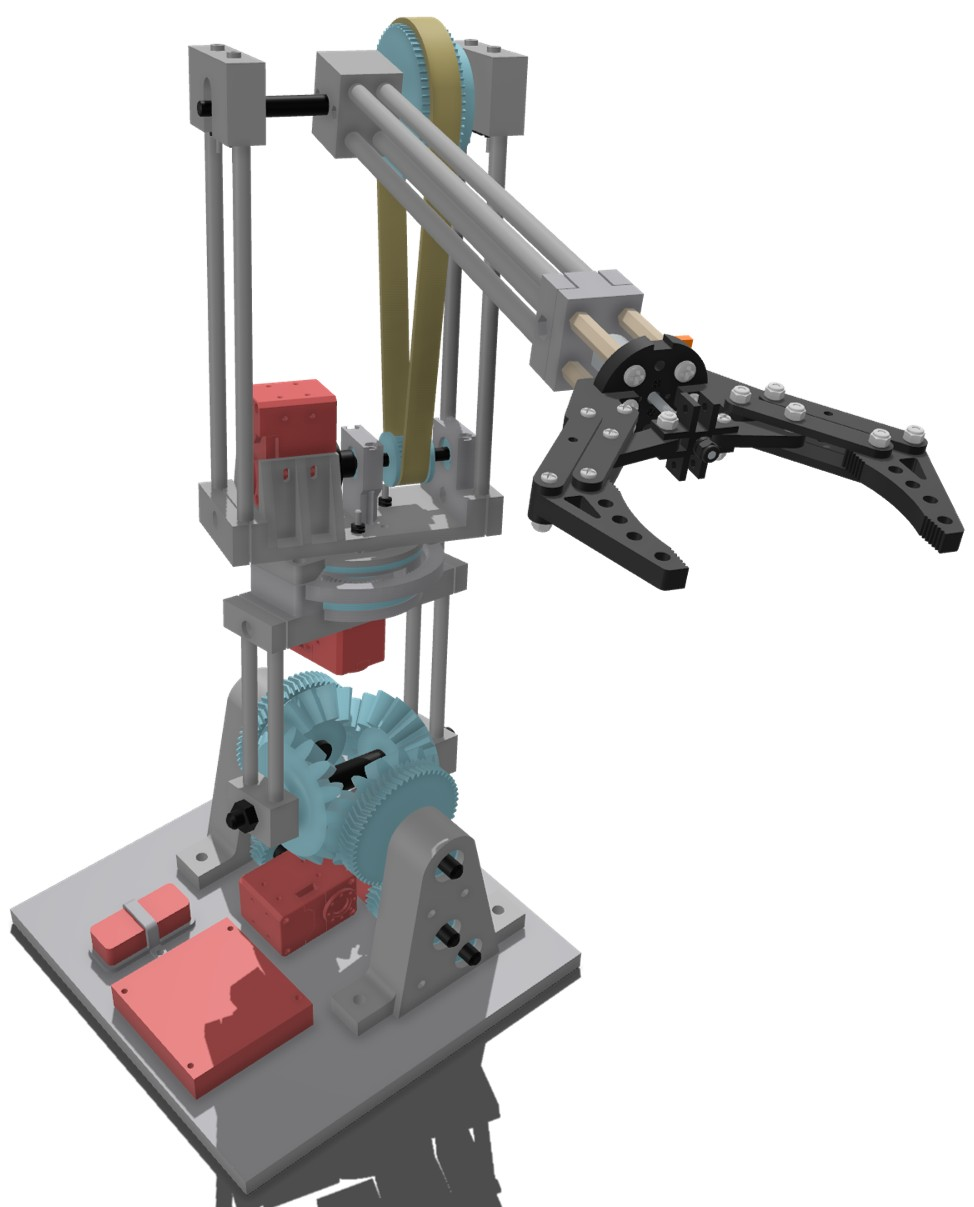
\includegraphics[width=0.8\linewidth]{images/robot_arm_final.jpg}
    \caption{Final version of the robotic arm with all hardware improvements modelled.}
    \label{fig:robot_arm_final}
\end{figure}

This version has been built in collaboration with the workshop of the institute, with the help of their machinery and expertise.
The built robotic arm can be seen in \autoref{fig:robot_arm_built}.
\begin{figure}[htbp]
    \centering
    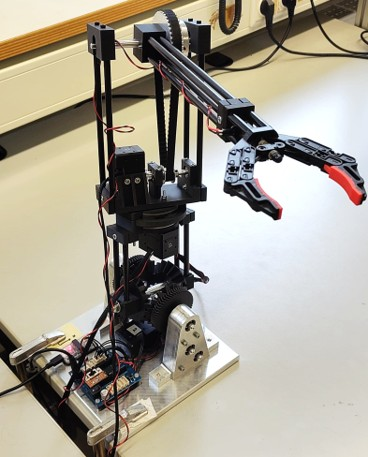
\includegraphics[width=0.8\linewidth]{images/robot_arm_built.jpg}
    \caption{Built version of the robotic arm with all hardware improvements implemented.}
    \label{fig:robot_arm_built}
\end{figure}